\subsection{Ejercicio 5}
\graphicspath{ {img/05} }

\subsubsection{Proceso para obtener certificado digital FNMT}

Lo primero que se debe hacer para obtener el certificado digital es entrar en la web de la Fábrica Nacional de Moneda y Timbre (FNMT). Una vez ahí, seleccionamos la opción “Obtener certificado digital como persona física”. Se verá en la pantalla la \ref{fig:web_ej5a}.

\begin{figure}[H]
    \centering
    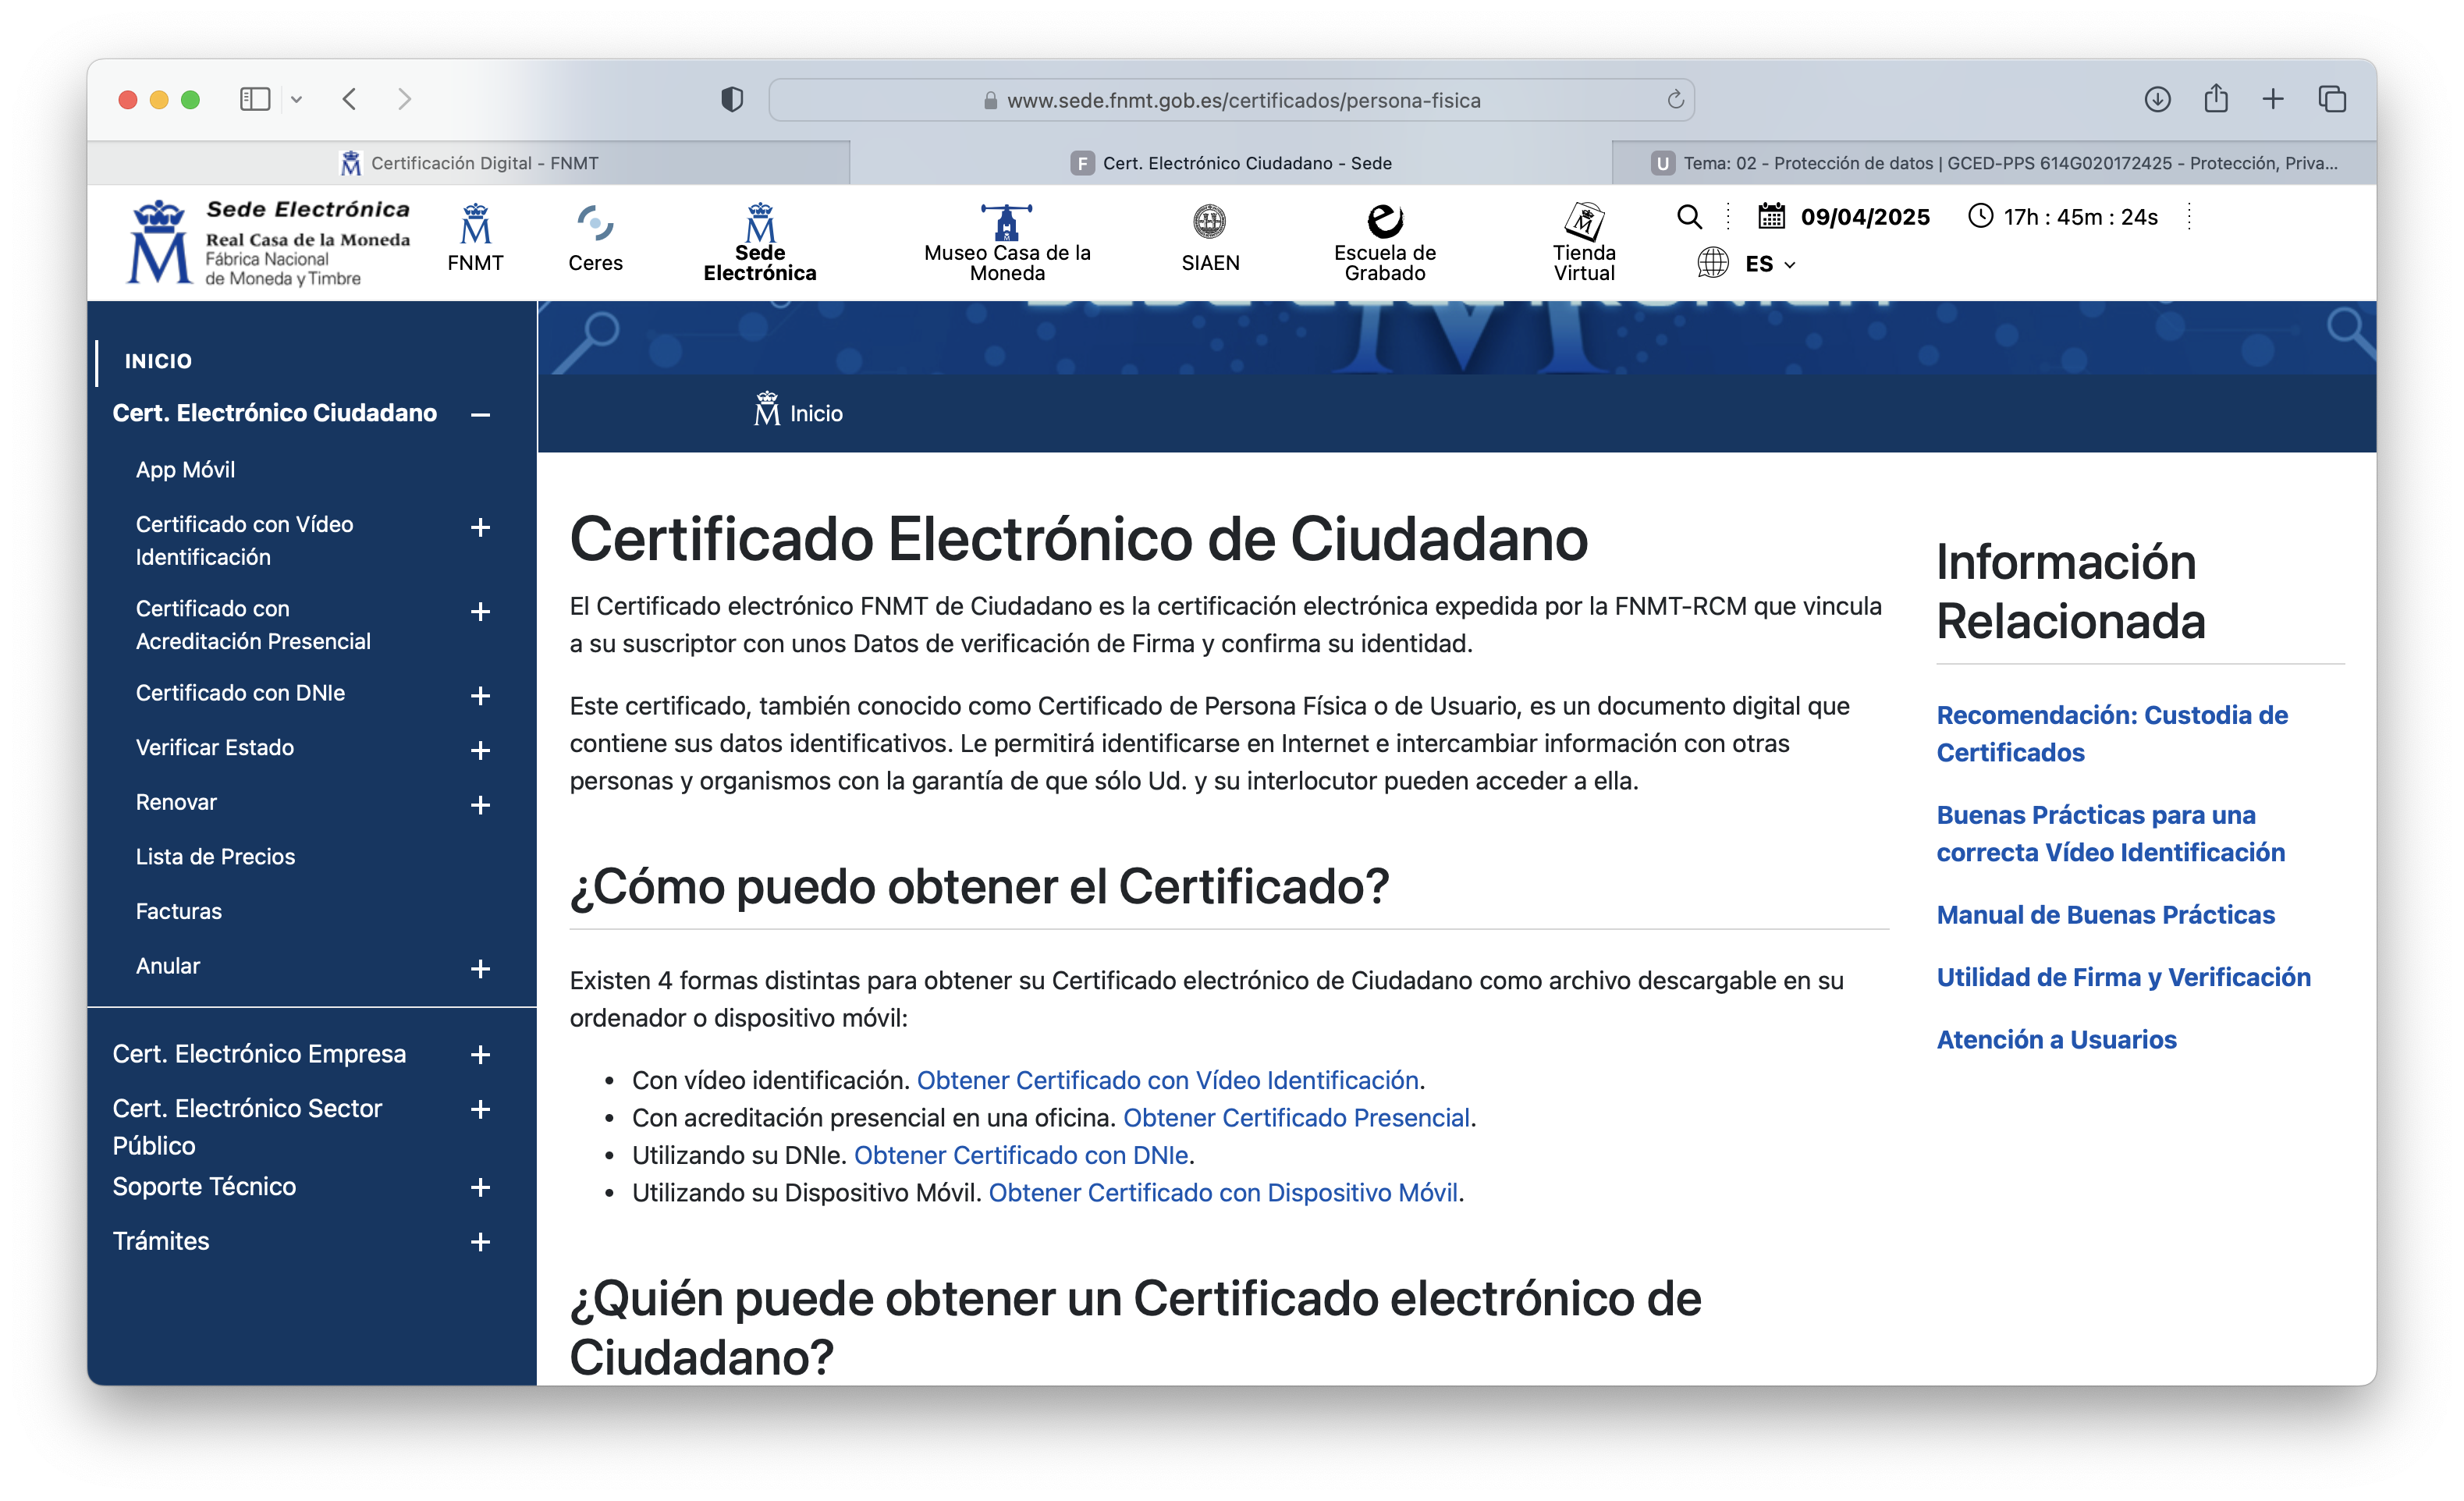
\includegraphics[width=\textwidth]{web_ej5a.png}
    \caption{Página inicio web FNMT}
    \label{fig:web_ej5a}
\end{figure}

En ella se ven las 4 formas a través de las que podemos conseguir el certificado. En nuestro caso, se eligió la opción de "Obtener certificado presencial". Una vez seleccionada la opción, como se ve en la \ref{fig:paso1}, se nos explican 4 pasos a seguir para obtener nuestro certificado.

El paso 1 consiste en una configuración previa. Se debe instalar una aplicación para solicitar las claves necesarias en la obtención de un certificado digital. Puede ser ejecutada en cualquier navegador y sistema Operativo. Una vez descargado e instalado el software no es necesario hacer nada, este se ejecutará cuando el navegador lo requiera. En la \ref{fig:instalacion_FNMT}, se ve el final de la instalación del software. En la propia instalación se crea la contraseña, necesaria para el paso final.

\begin{figure}[H]
    \centering
    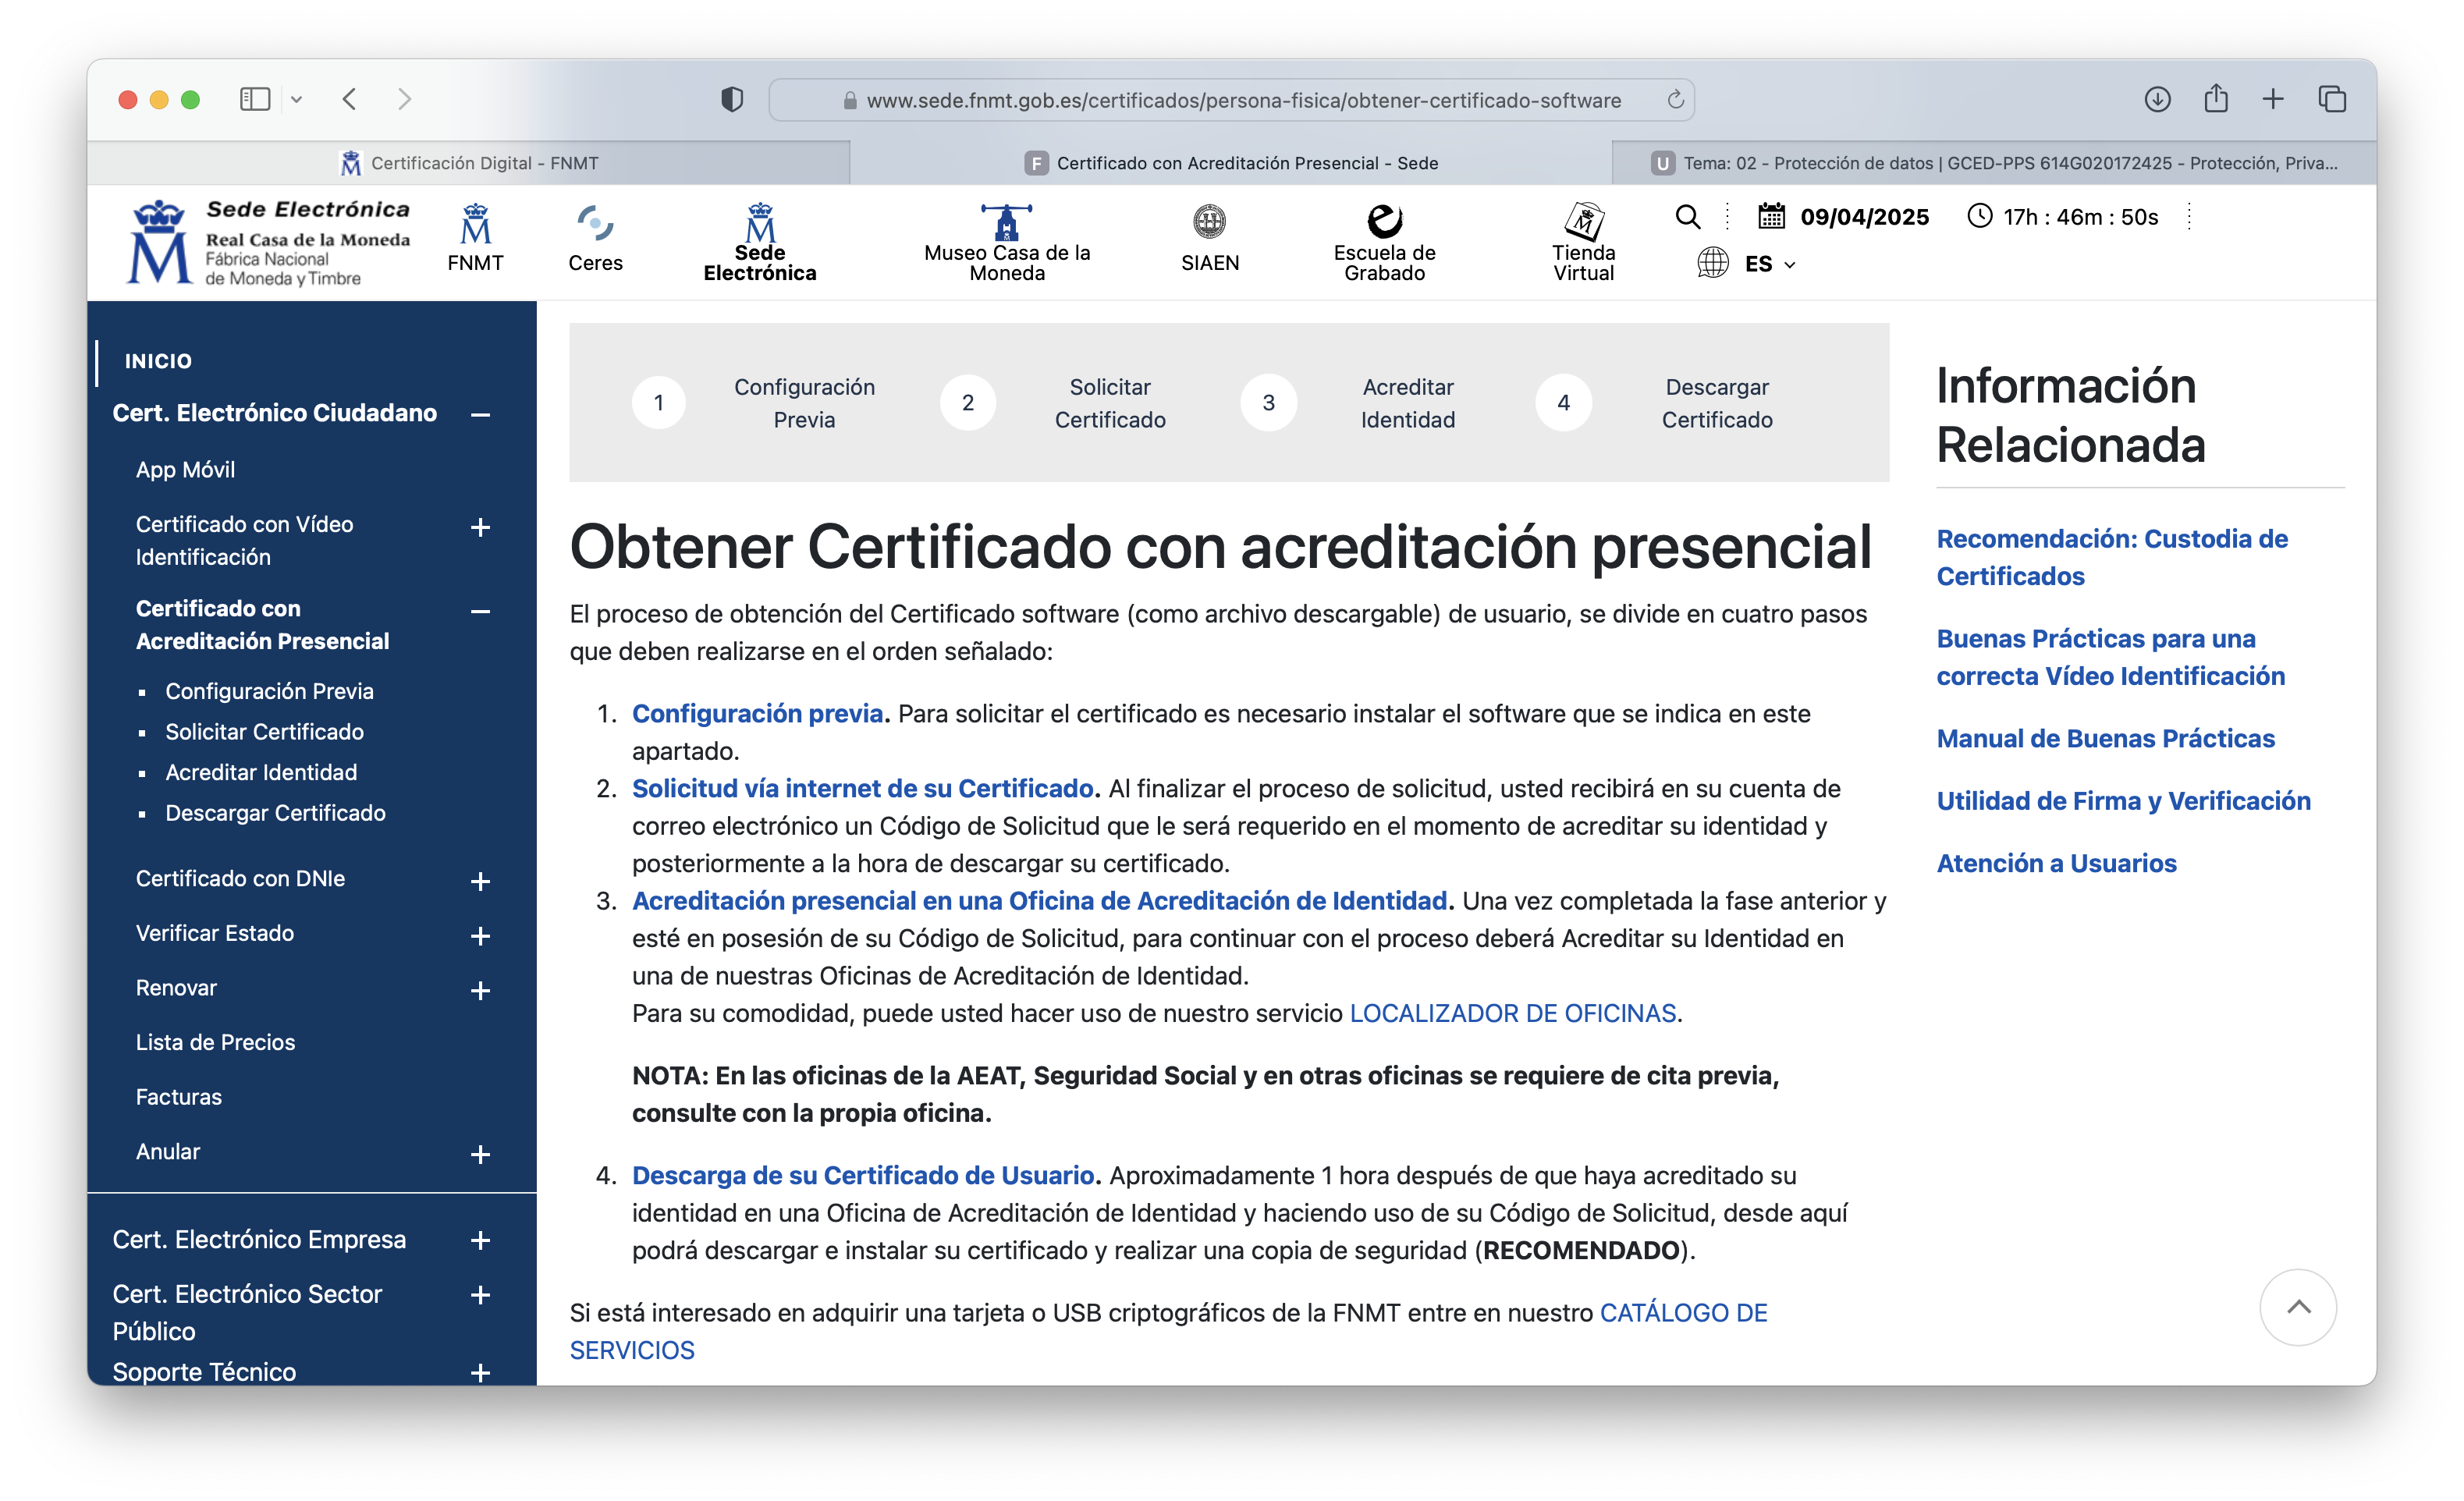
\includegraphics[width=0.9\textwidth]{paso1_ej5a.png}
    \caption{Paso 1}
    \label{fig:paso1}
\end{figure}

\begin{figure}[H]
    \centering
    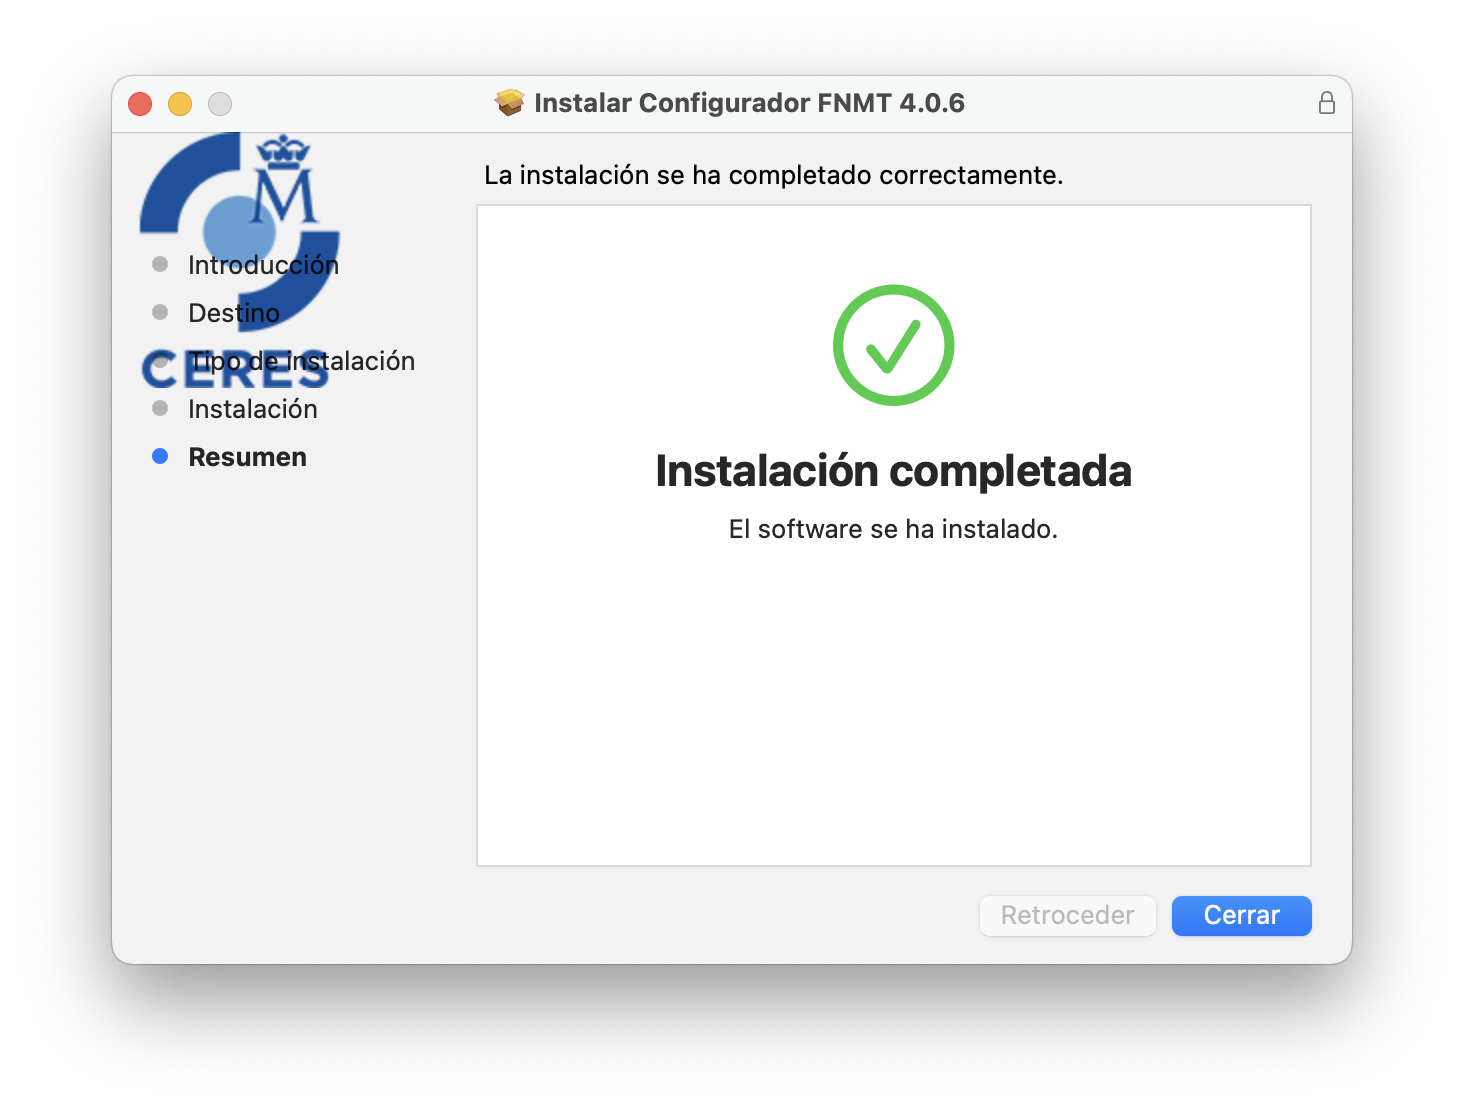
\includegraphics[width=0.9\textwidth]{instalacion_FNMT_ej5a.png}
    \caption{Instalación software FNMT}
    \label{fig:instalacion_FNMT}
\end{figure}

Una vez instalado el software, proseguimos con el paso 2. En este paso debemos cubrir un formulario para solicitar el certificado. En la \ref{fig:paso2} se ve el formulario a cubrir. Tras la solicitud, se recibe un correo electrónico que incluye un código de solicitud.

\begin{figure}[H]
    \centering
    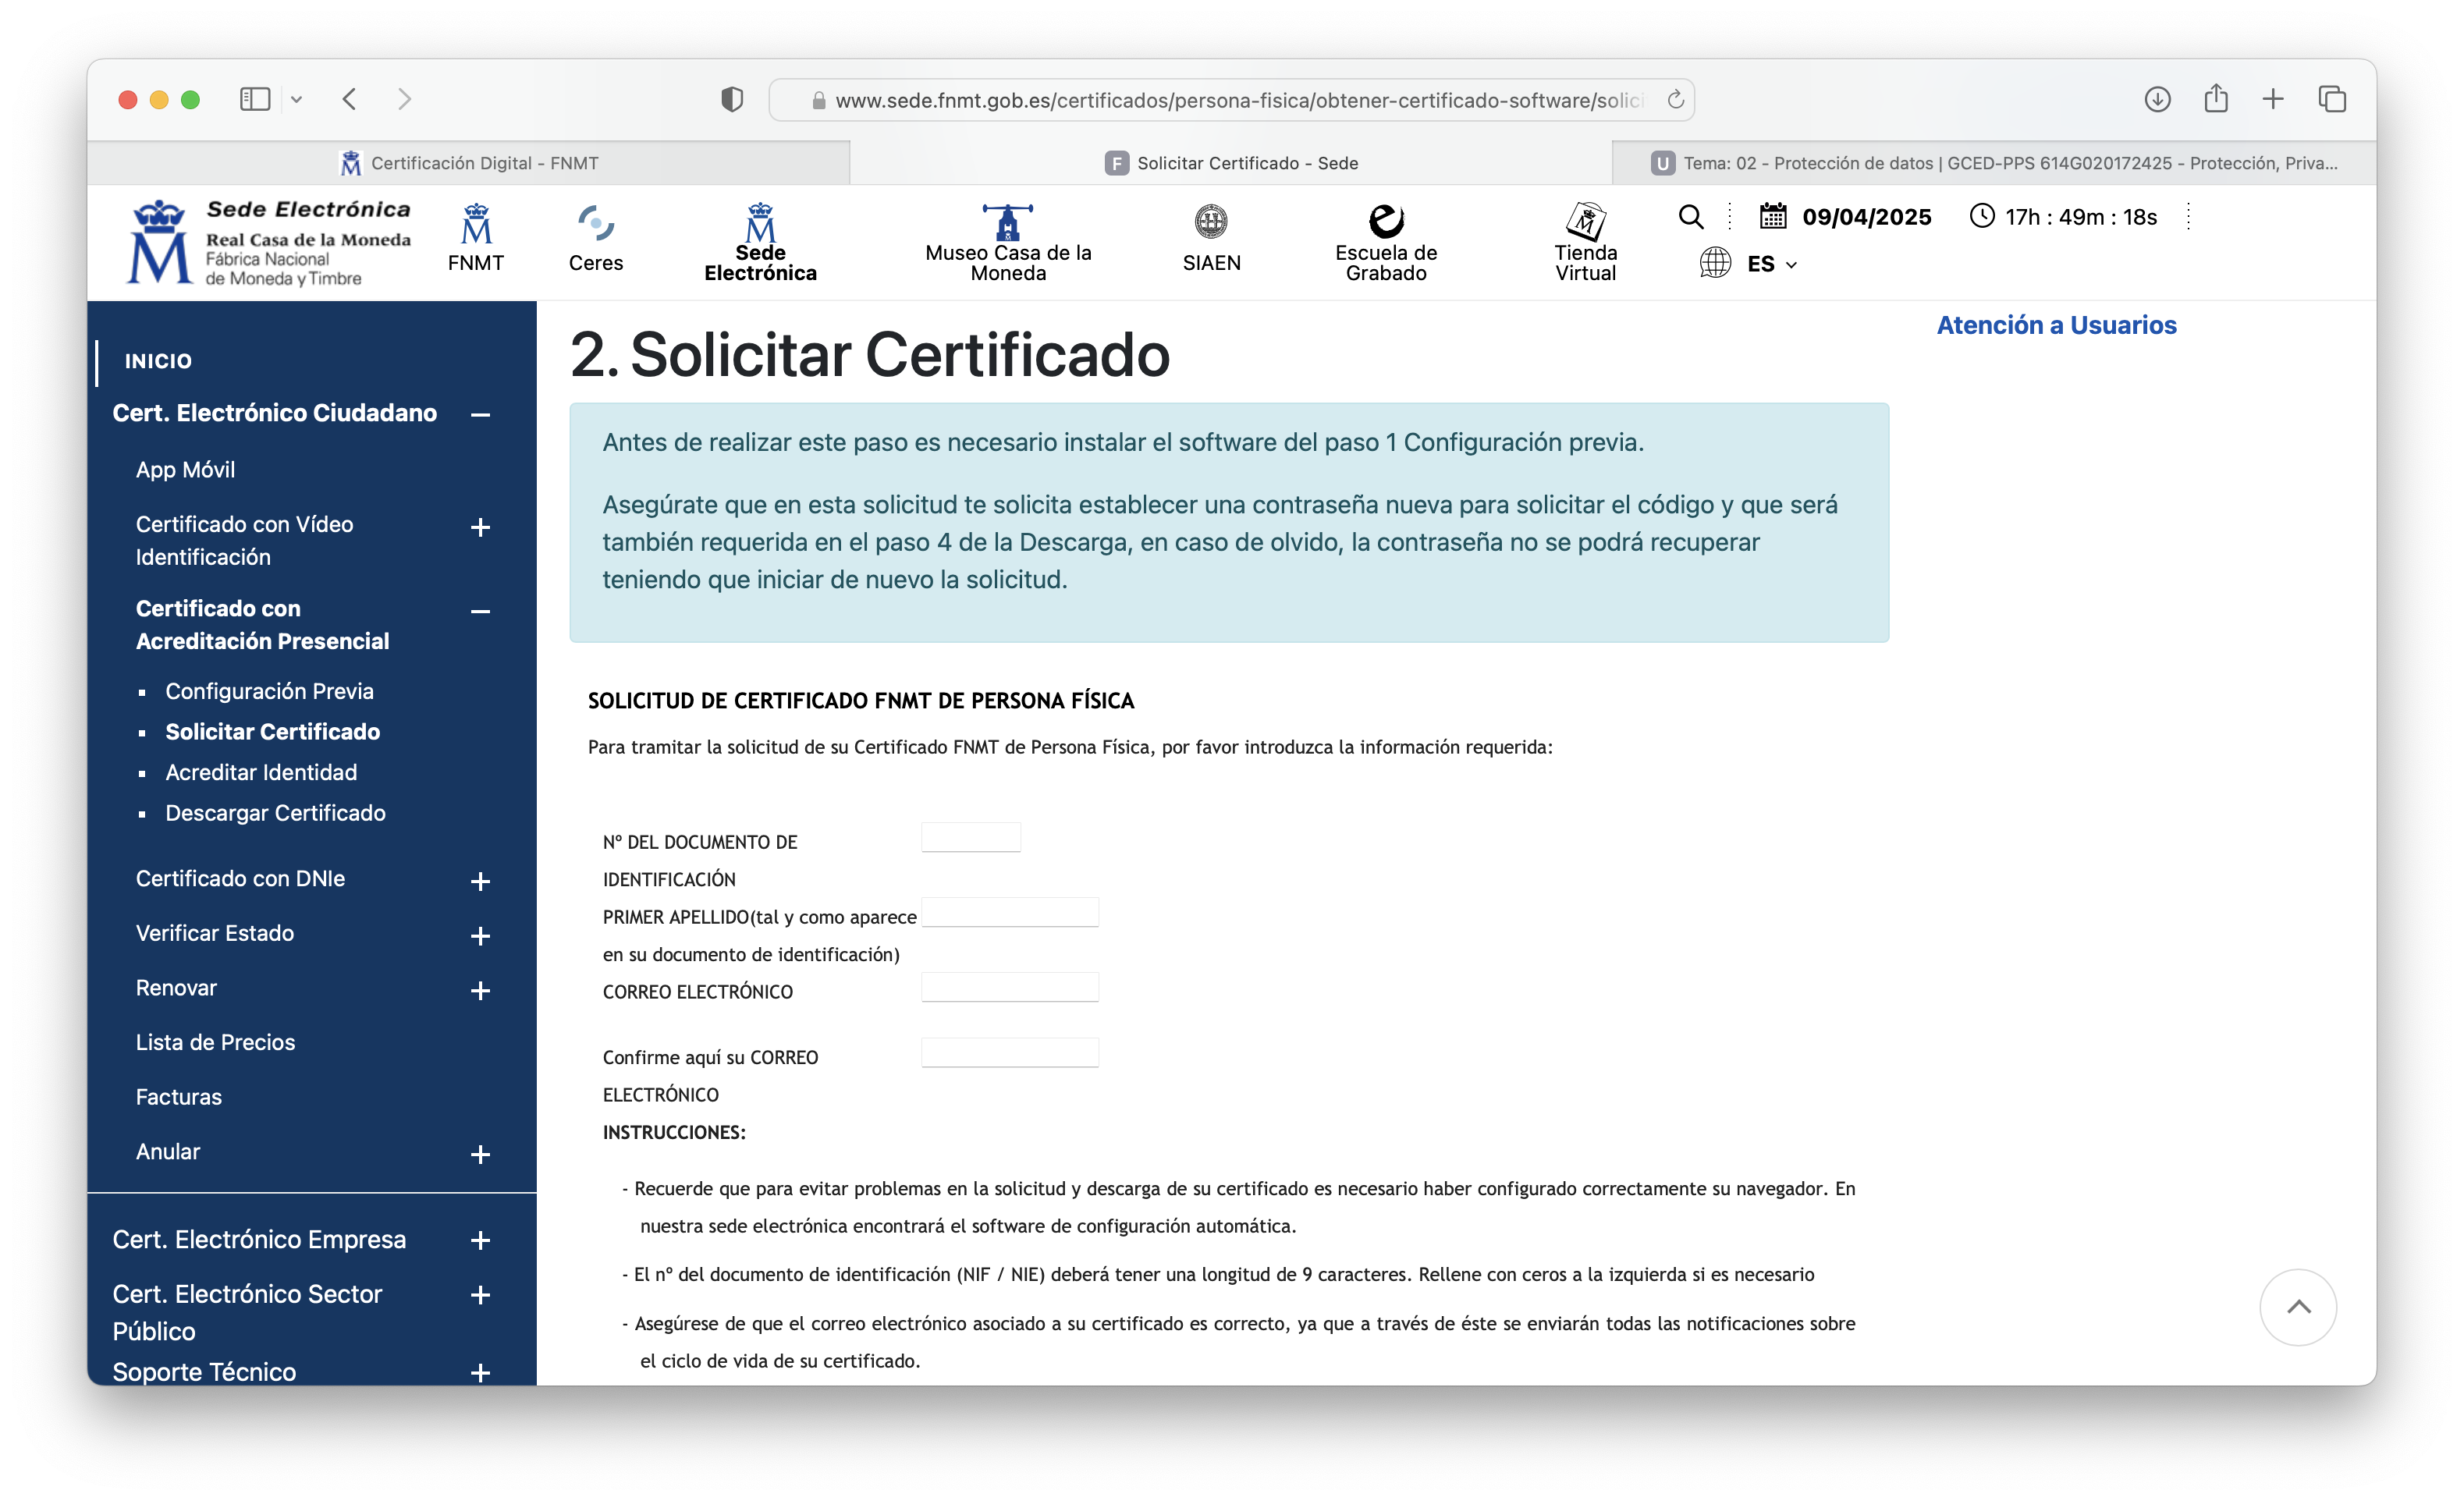
\includegraphics[width=0.8\textwidth]{paso2_ej5a.png}
    \caption{Paso 2}
    \label{fig:paso2}
\end{figure}

El tercer paso consiste en acudir presencialmente a una oficina de registro habilitada con nuestro DNI físico y el código de solicitud obtenido en el correo electrónico del paso anterior. Allí, nos identificaron presencialmente y validaron nuestra identidad. En la página web de la FNMT se puede encontrar el mapa de la \ref{fig:mapa}, con las oficinas a las que podemos acudir, en nuestro caso, hacienda. Tras la cita, recibiremos otro correo electrónico.

\begin{figure}[H]
    \centering
    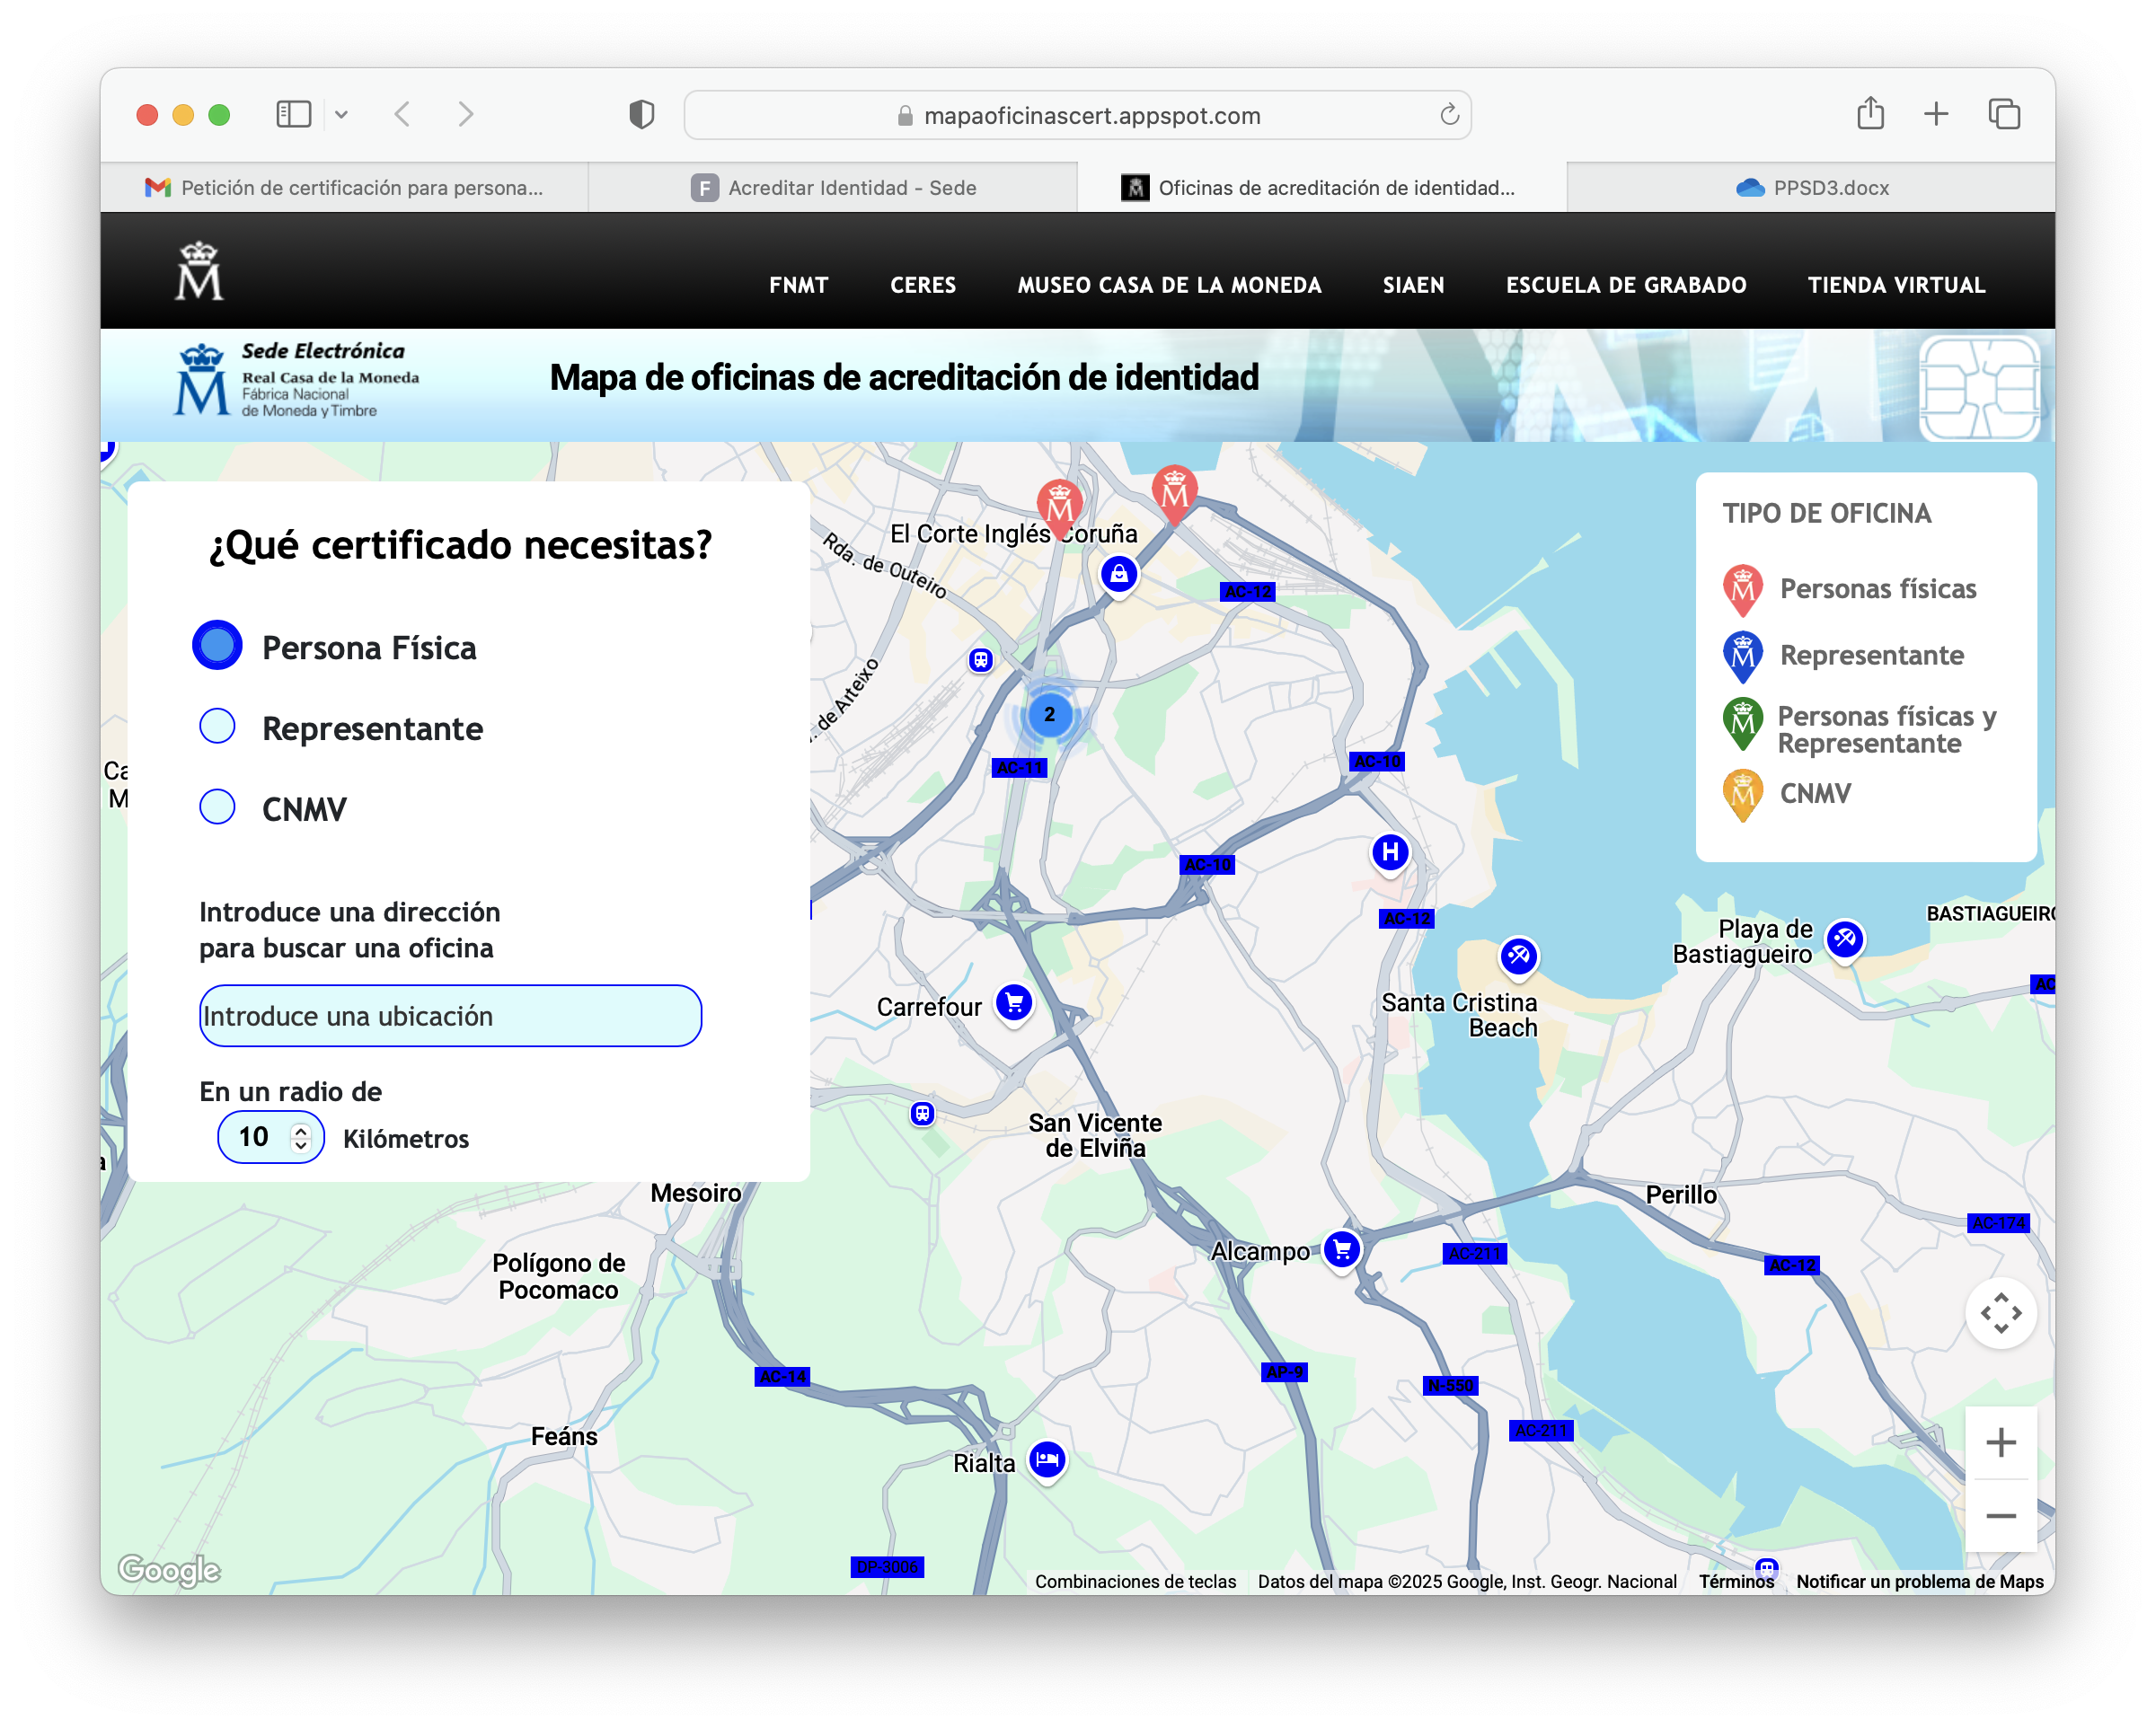
\includegraphics[width=0.8\textwidth]{mapa_ej5a.png}
    \caption{Mapa oficinas de acreditación}
    \label{fig:mapa}
\end{figure}

El último paso consiste en descargar el certificado en el mismo navegador y equipo con el que se hizo la solicitud. En el correo electrónico recibido tras acudir a hacienda, se nos proporciona la confirmación de nuestra solicitud, así como el enlace al formulario de la \ref{fig:paso4}. Una vez cubierto, el navegador instala el certificado, vinculando la clave privada local con el certificado emitido por la FNMT. Se debe ver un mensaje como el de la \ref{fig:fin_instalacion}. Es recomendable descargar el certificado en nuestro dispositivo.

\begin{figure}[H]
    \centering
    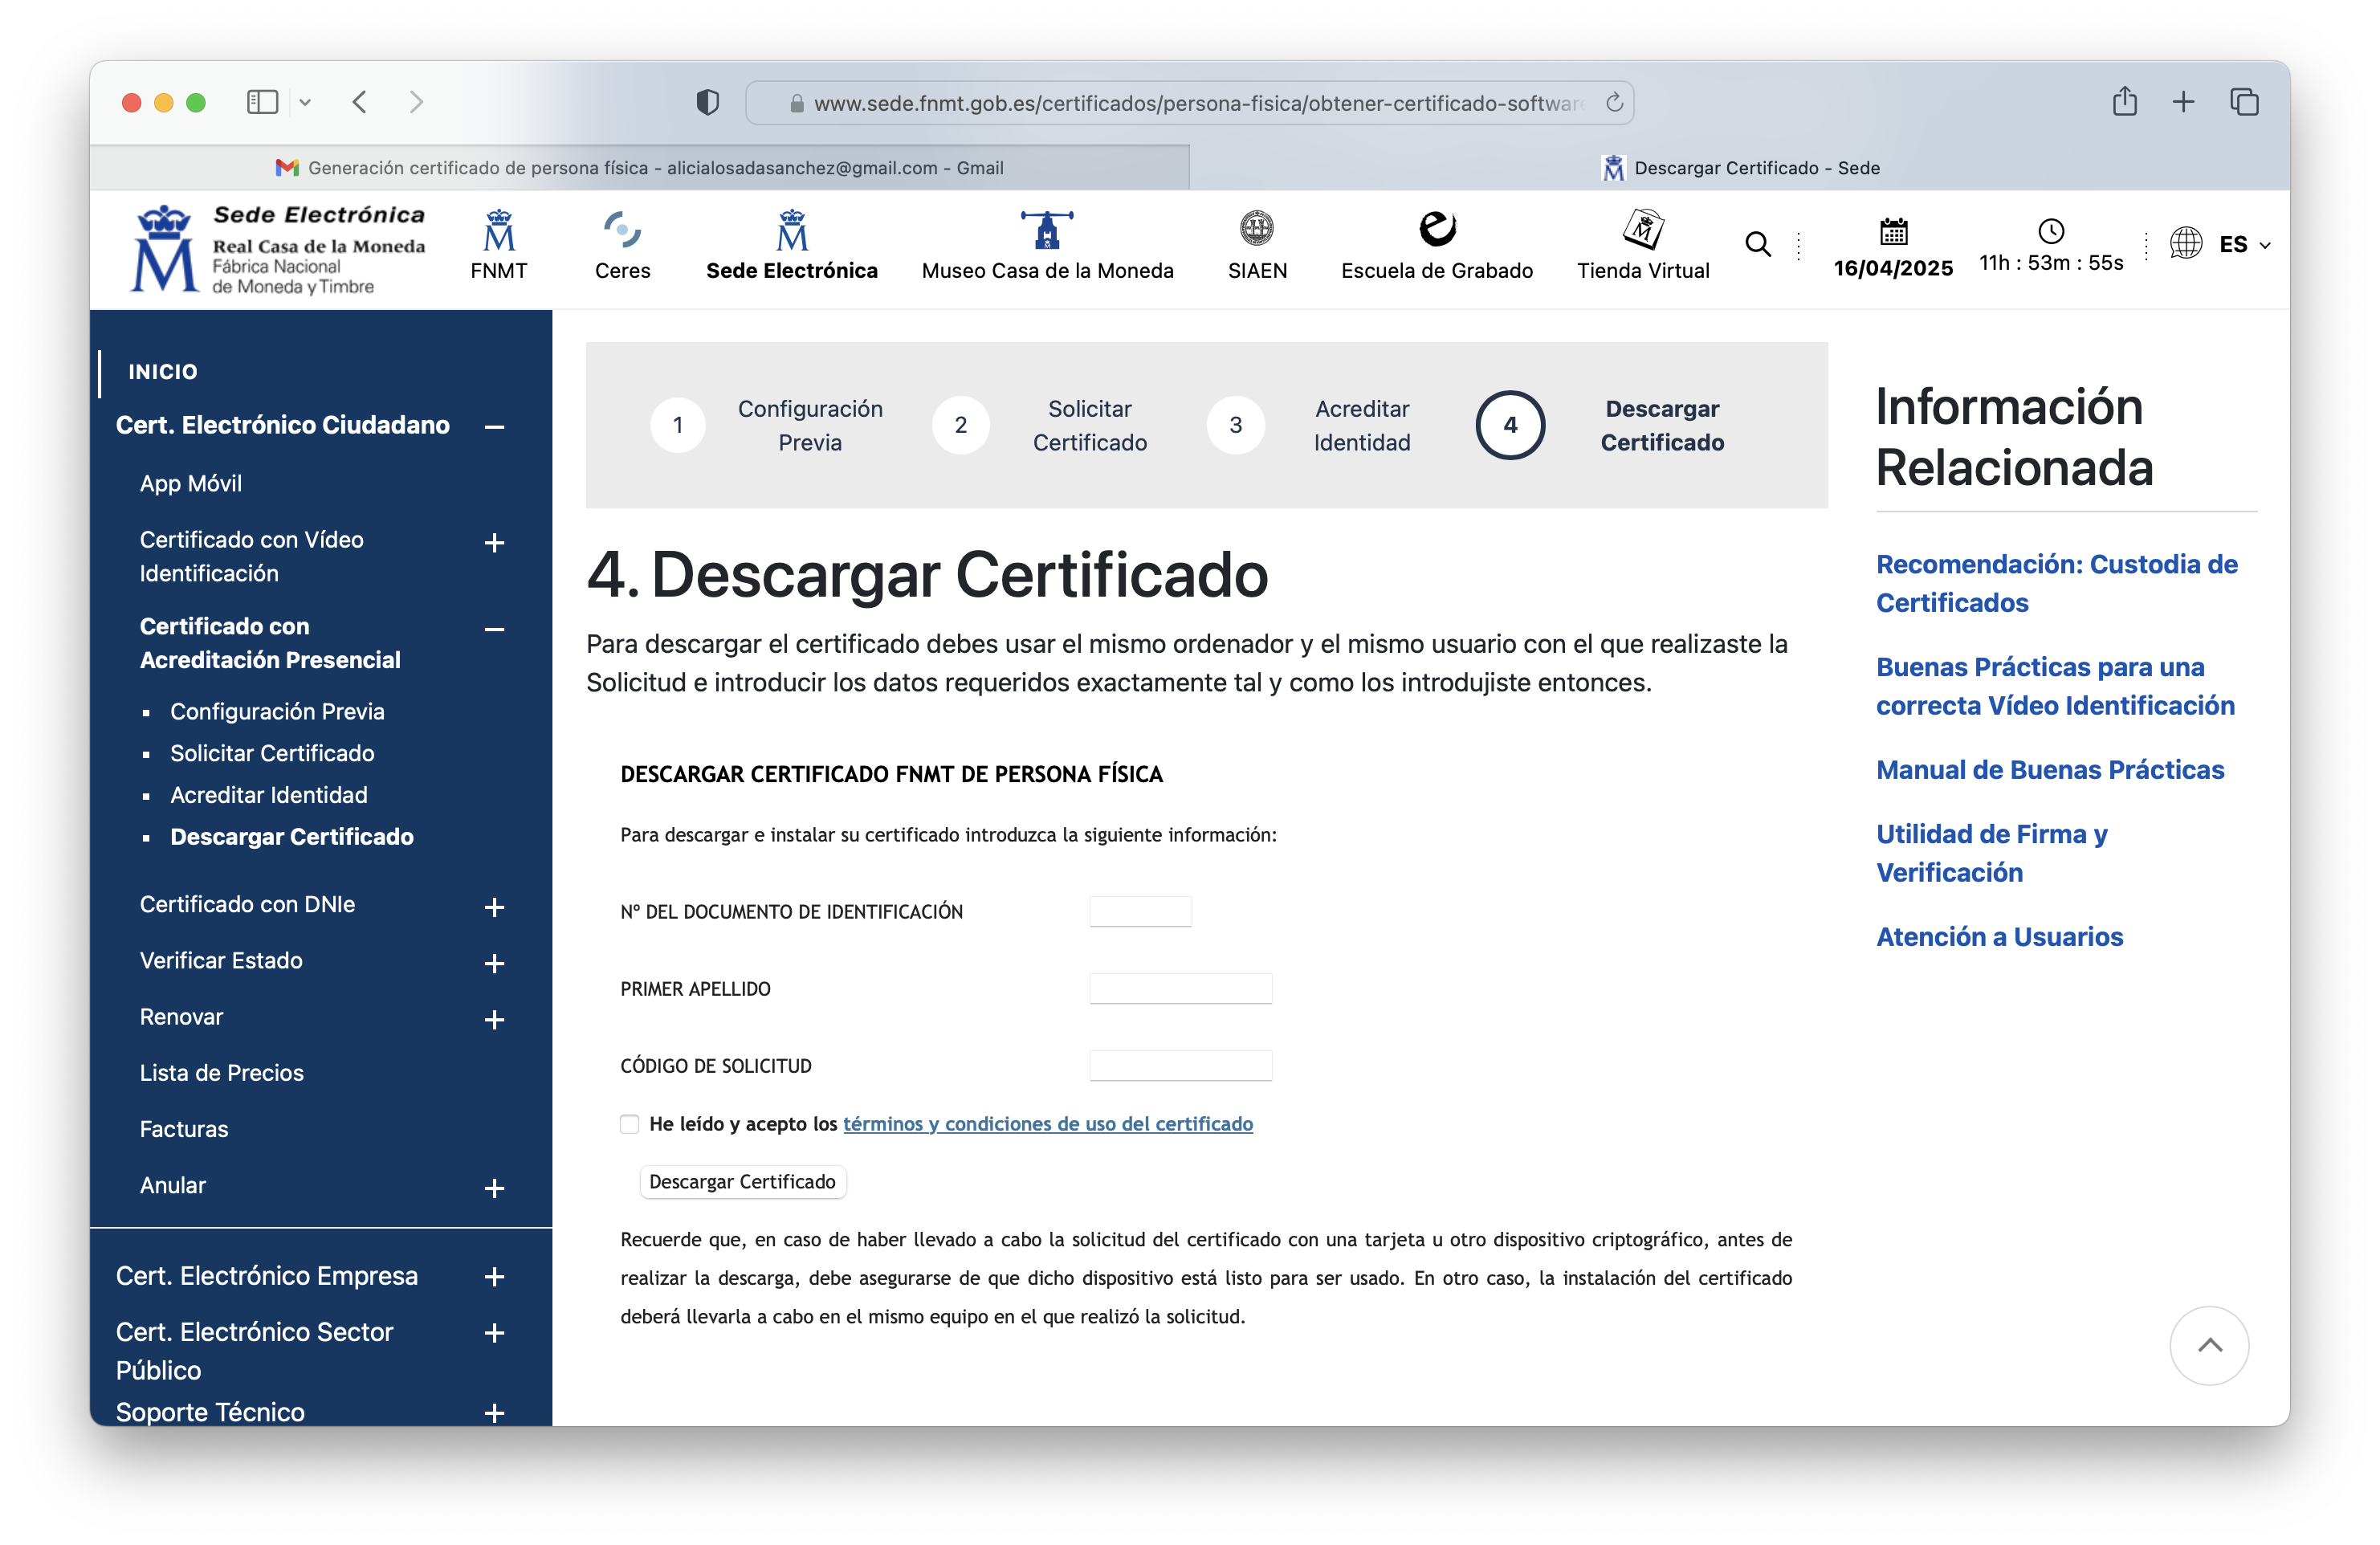
\includegraphics[width=0.8\textwidth]{paso4_ej5a.png}
    \caption{Paso 4}
    \label{fig:paso4}
\end{figure}

\begin{figure}[H]
    \centering
    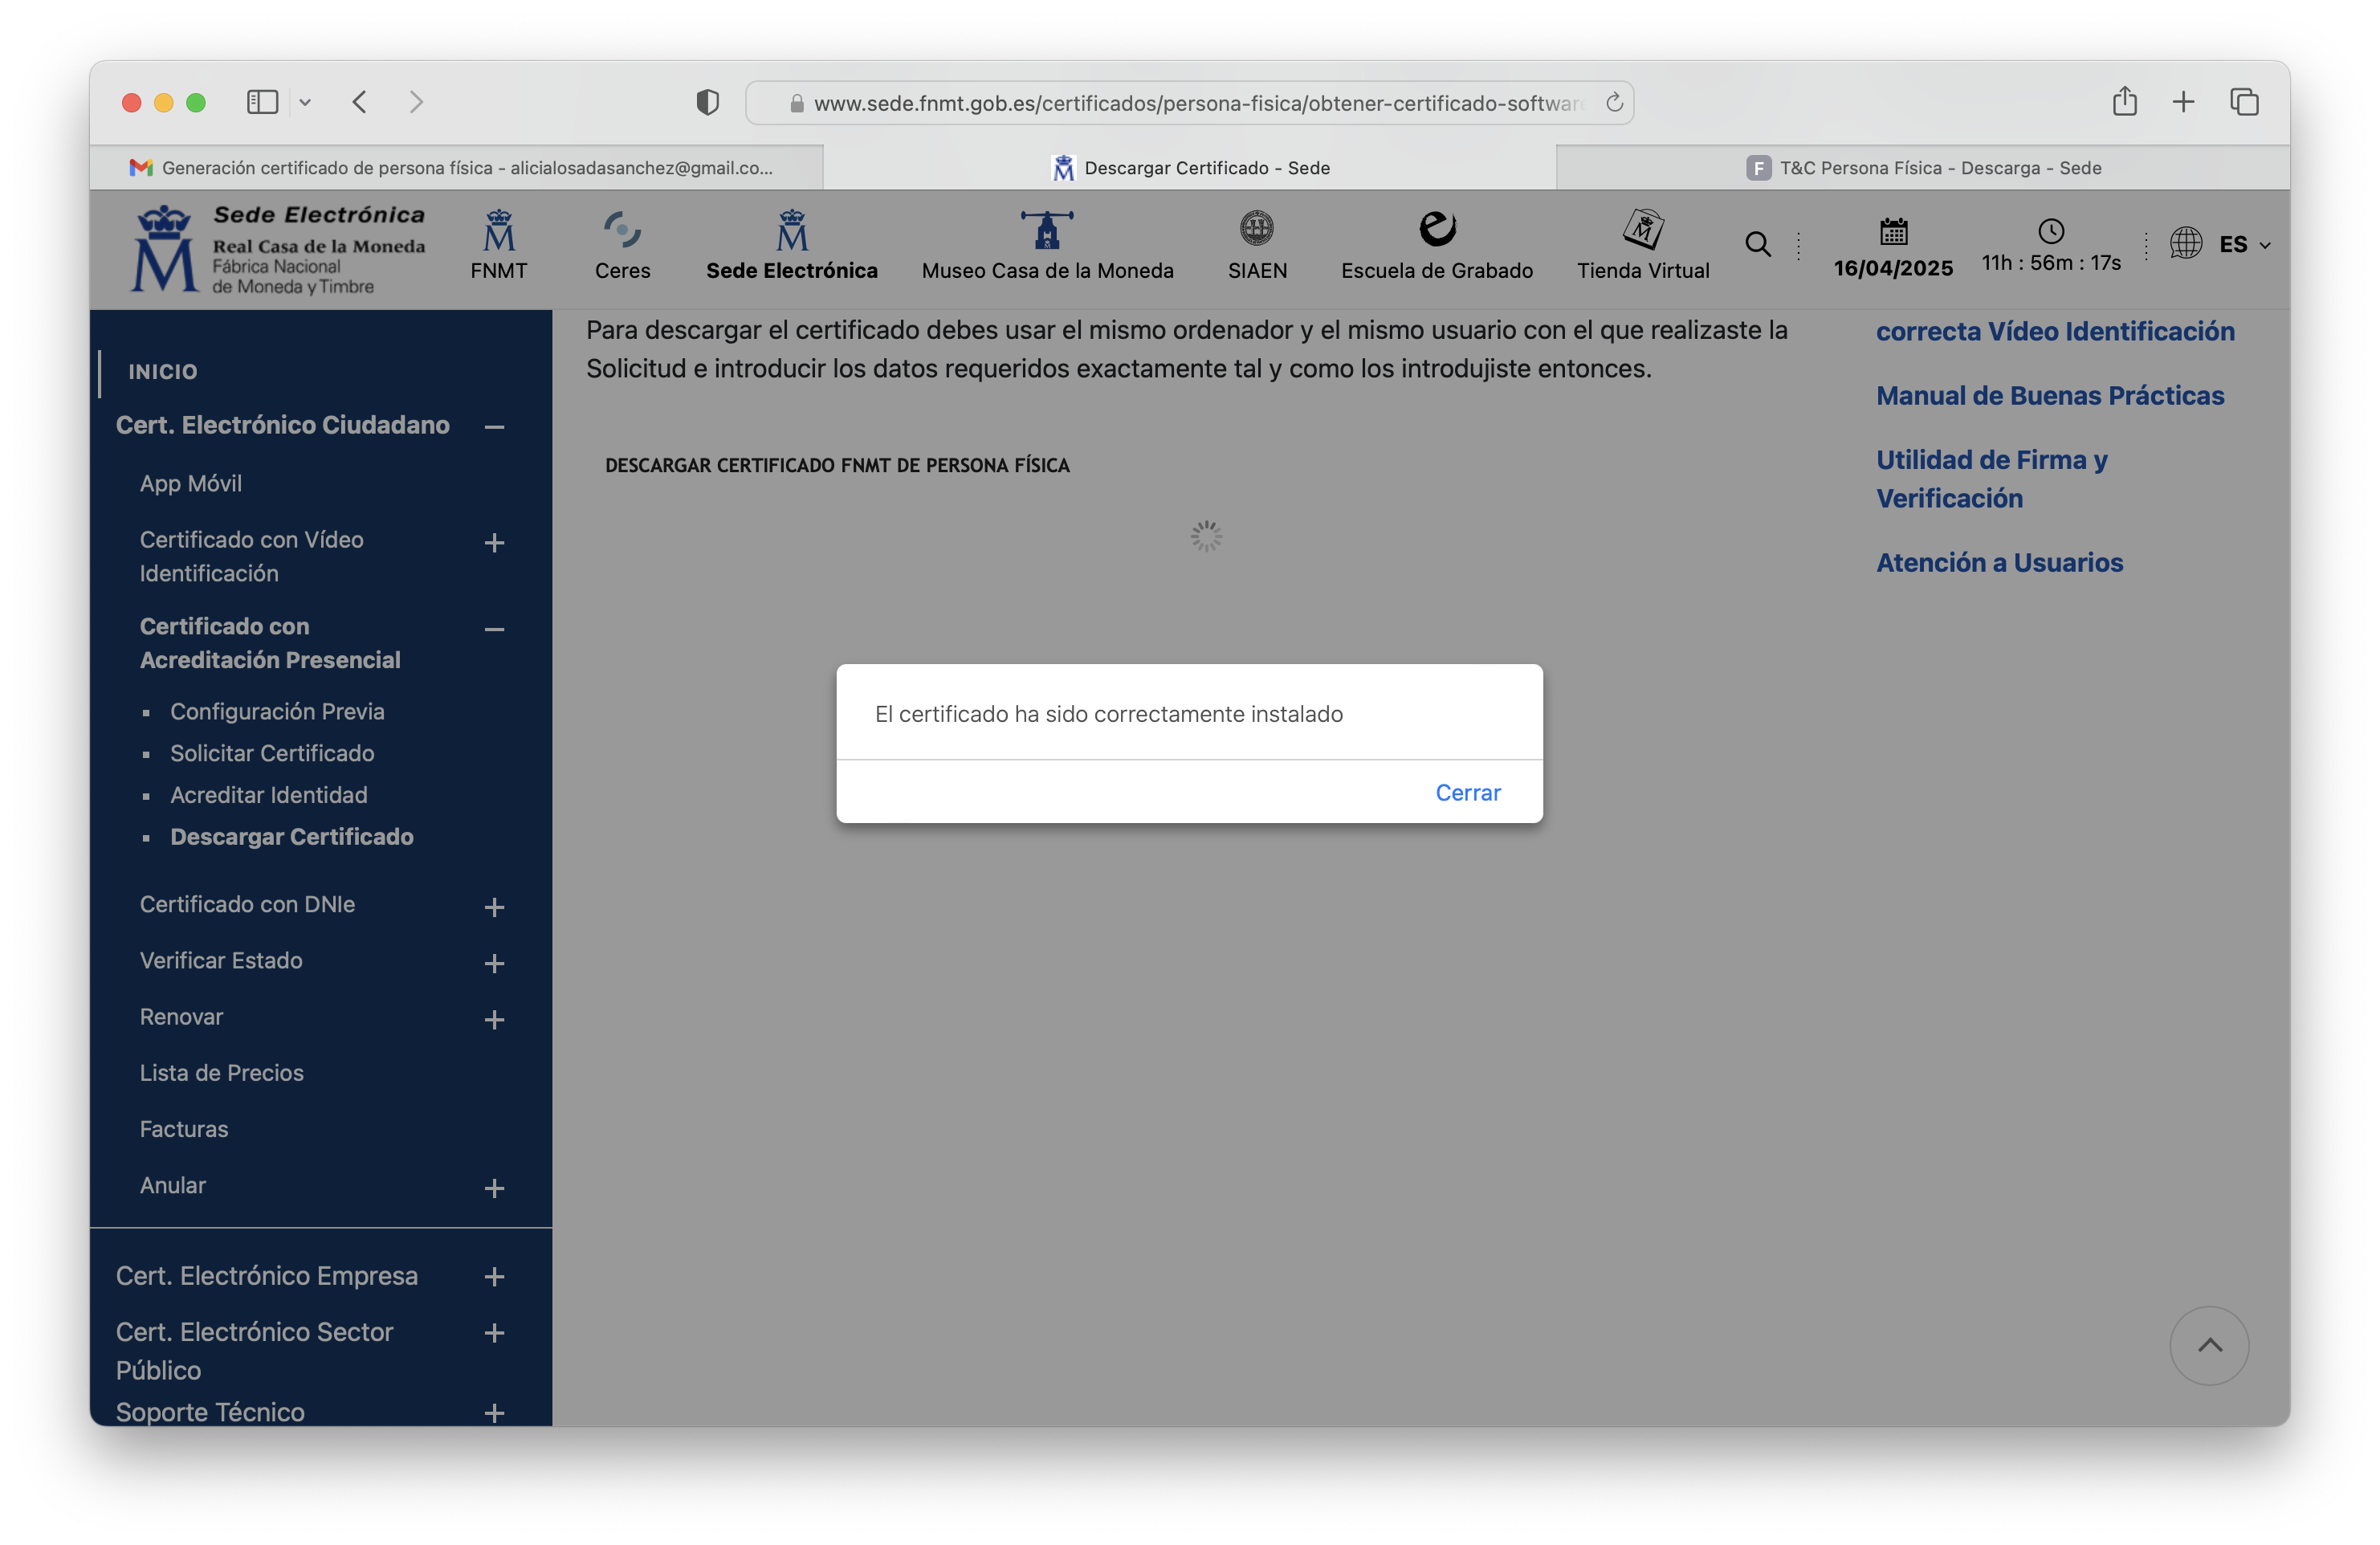
\includegraphics[width=0.8\textwidth]{fin_instalacion_ej5a.png}
    \caption{Fin instalación certificado}
    \label{fig:fin_instalacion}
\end{figure}

Las claves se generan en el propio navegador del usuario en el momento en que se realiza la solicitud del certificado digital en la web de la FNMT. Específicamente, el navegador crea un par de claves: una clave pública, que se envía a la Autoridad Certificadora (CA), y una clave privada, que nunca abandona el equipo del usuario.

Esta clave privada se almacena localmente en el almacén de certificados del navegador o del sistema operativo, dependiendo del navegador utilizado. Por ejemplo, en Firefox se guarda en su propio almacén interno, mientras que en navegadores como Chrome o Edge en Windows, se almacena en el almacén de certificados del sistema operativo.

\subsubsection{Certificado formato PKCS 7}

Para poder obtener el certificado de clave pública en formato PKCS 7, se deben utilizar los siguientes comandos.

Primero, debemos pasar el fichero '.p12' a un fichero con formato '.pem', que será utilizado en el siguiente apartado. Para ello, necesitamos el siguiente comando:

\begin{minted}[
    frame=single,
    framesep=8pt,
    breaklines,
    bgcolor=bgGray
]{bash}
    openssl pkcs12 -in certificado.p12 -clcerts -nokeys -out certificado.pem
\end{minted}

Posteriormente, para obtener el certificado en formato '.p7b', debemos utilizar el siguiente comando:

\begin{minted}[
    frame=single,
    framesep=8pt,
    breaklines,
    bgcolor=bgGray
]{bash}
    openssl crl2pkcs7 -nocrl -certfile certificado.pem -out certficado.p7b
\end{minted}

\subsubsection{Análisis campos clave pública OpenSSL}

\begin{figure}[H]
    \centering
    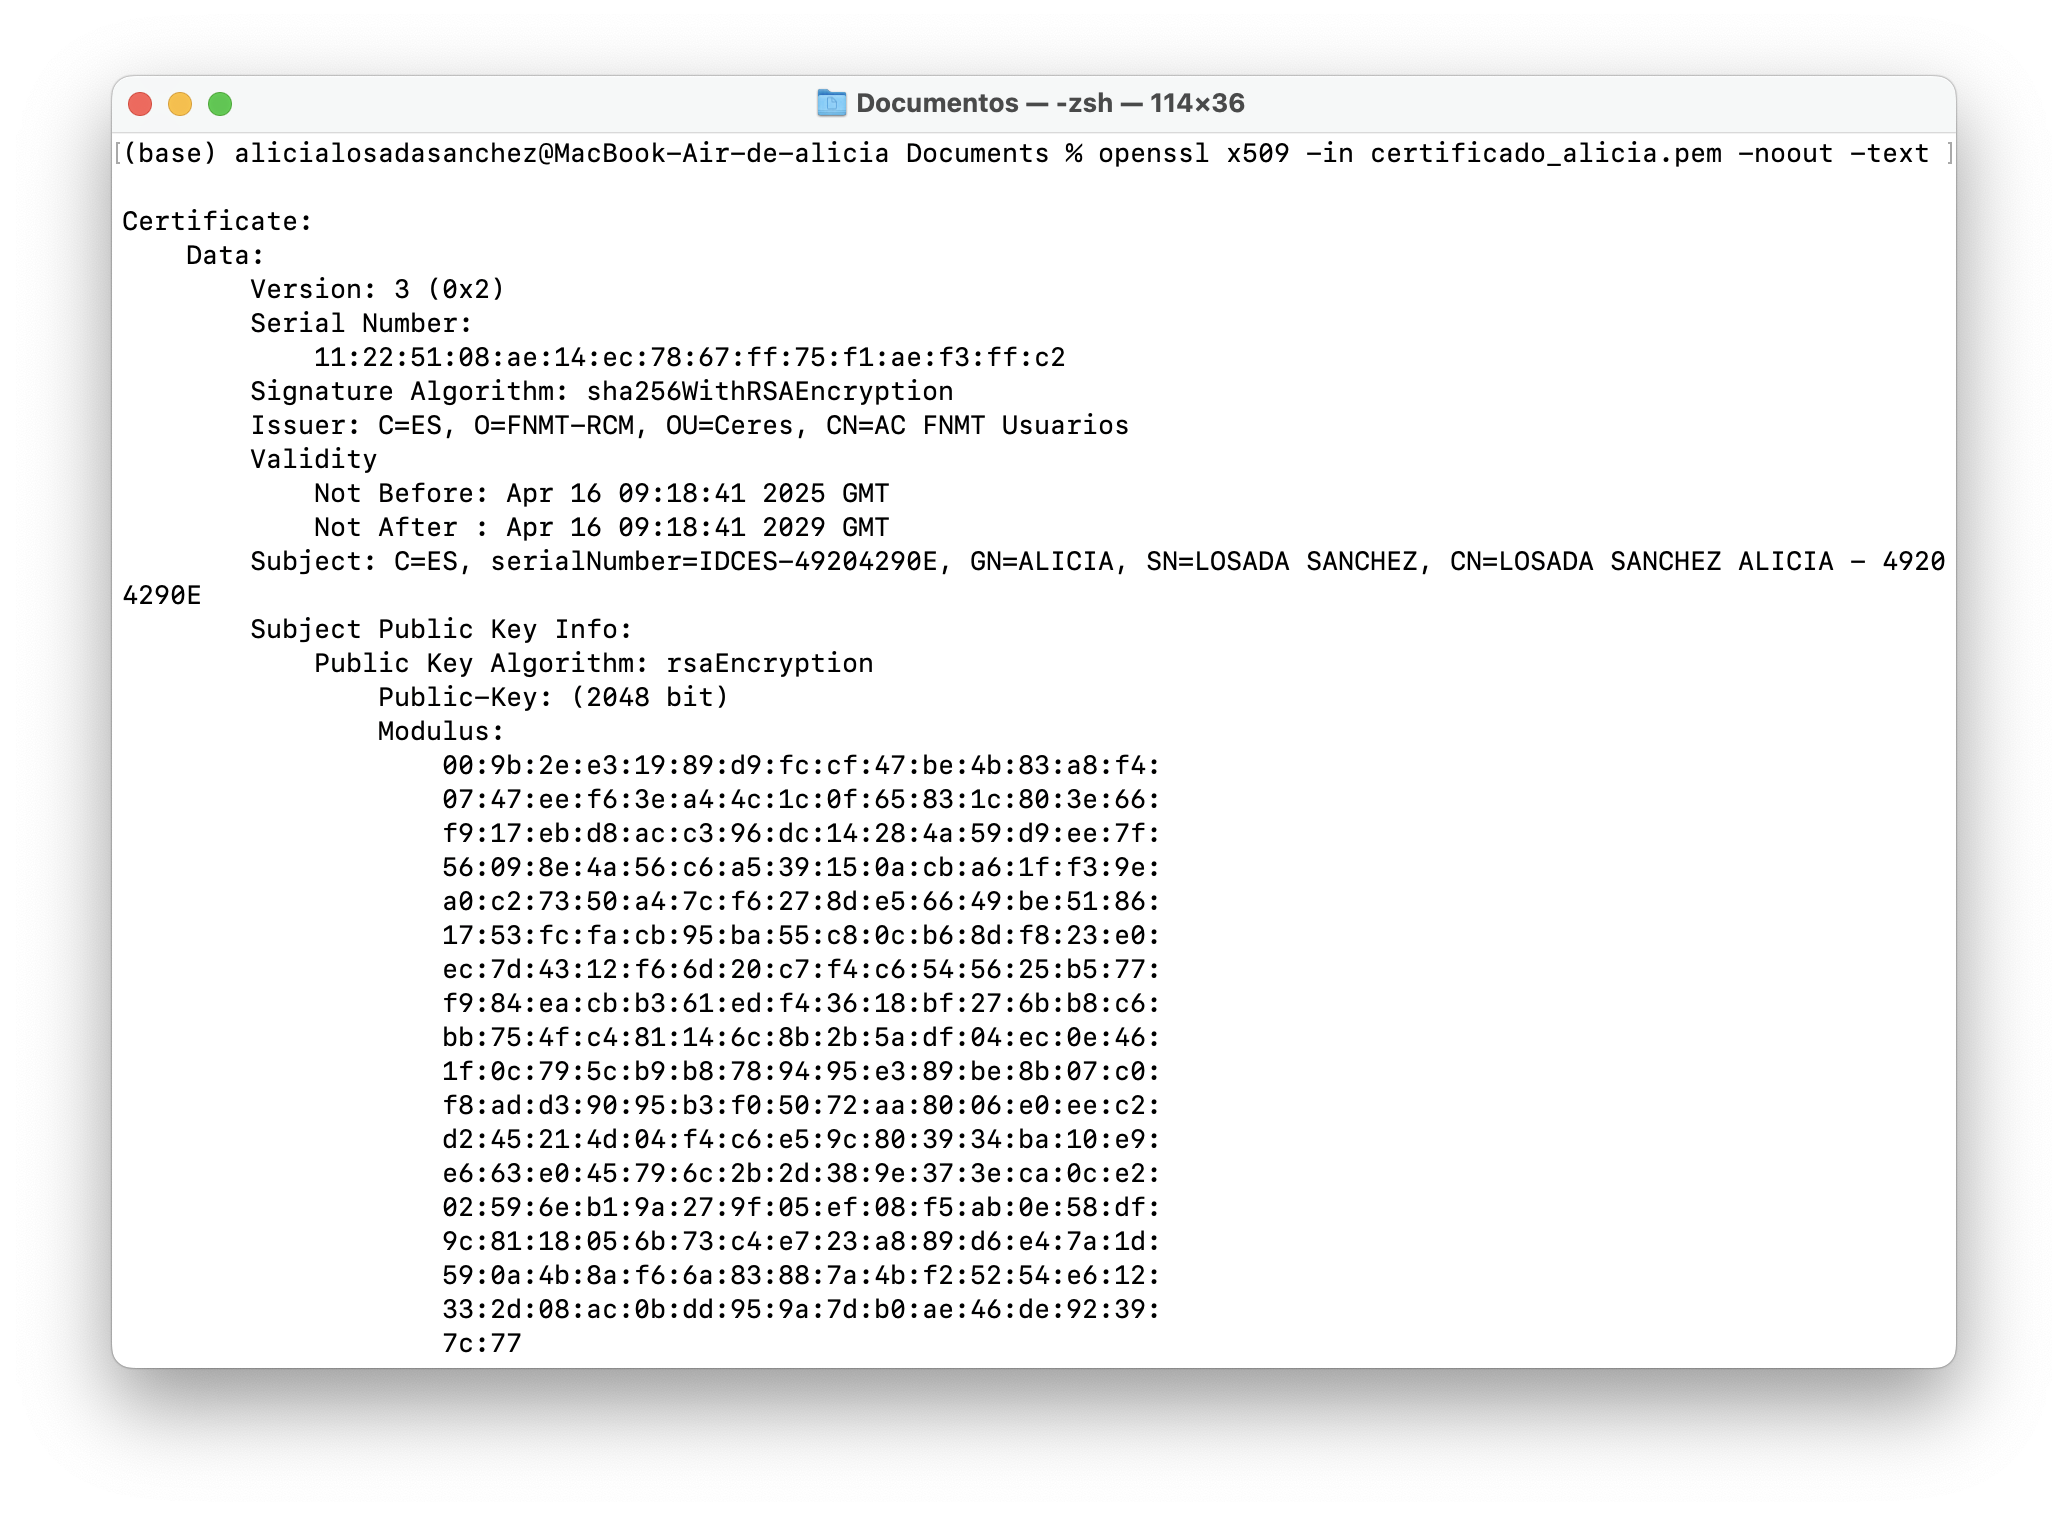
\includegraphics[width=0.8\textwidth]{apartadoc_1.png}
    \caption{Parte 1 campos clave pública}
    \label{fig:apartadoc_1}
\end{figure}

\begin{figure}[H]
    \centering
    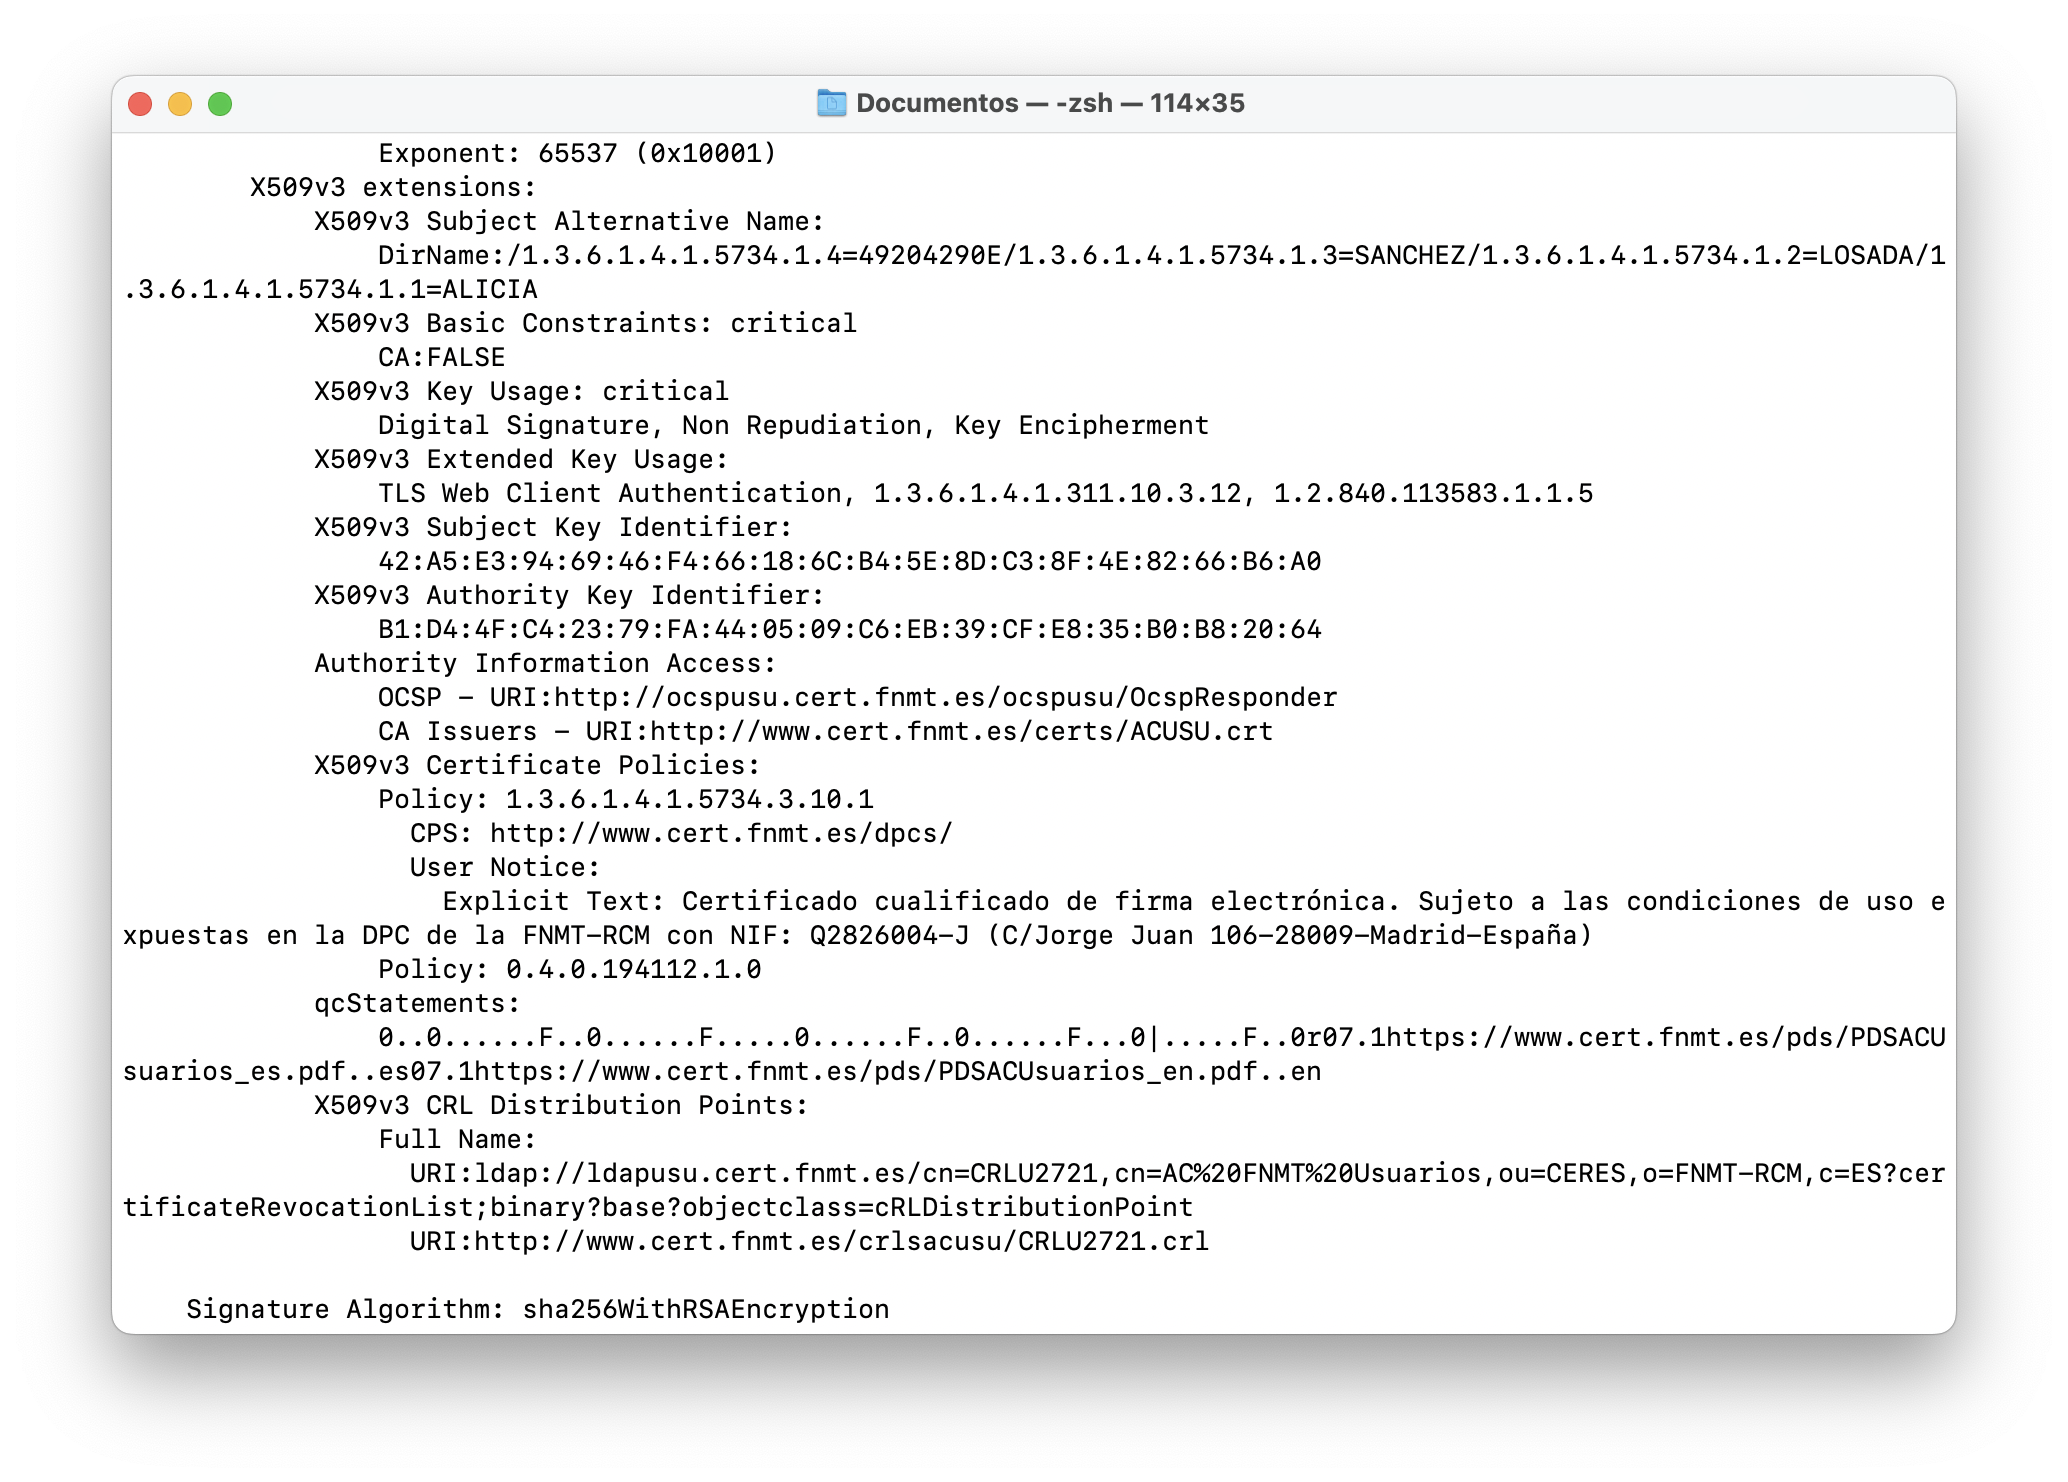
\includegraphics[width=0.8\textwidth]{apartadoc_2.png}
    \caption{Parte 2 campos clave pública}
    \label{fig:apartadoc_2}
\end{figure}

\begin{figure}[H]
    \centering
    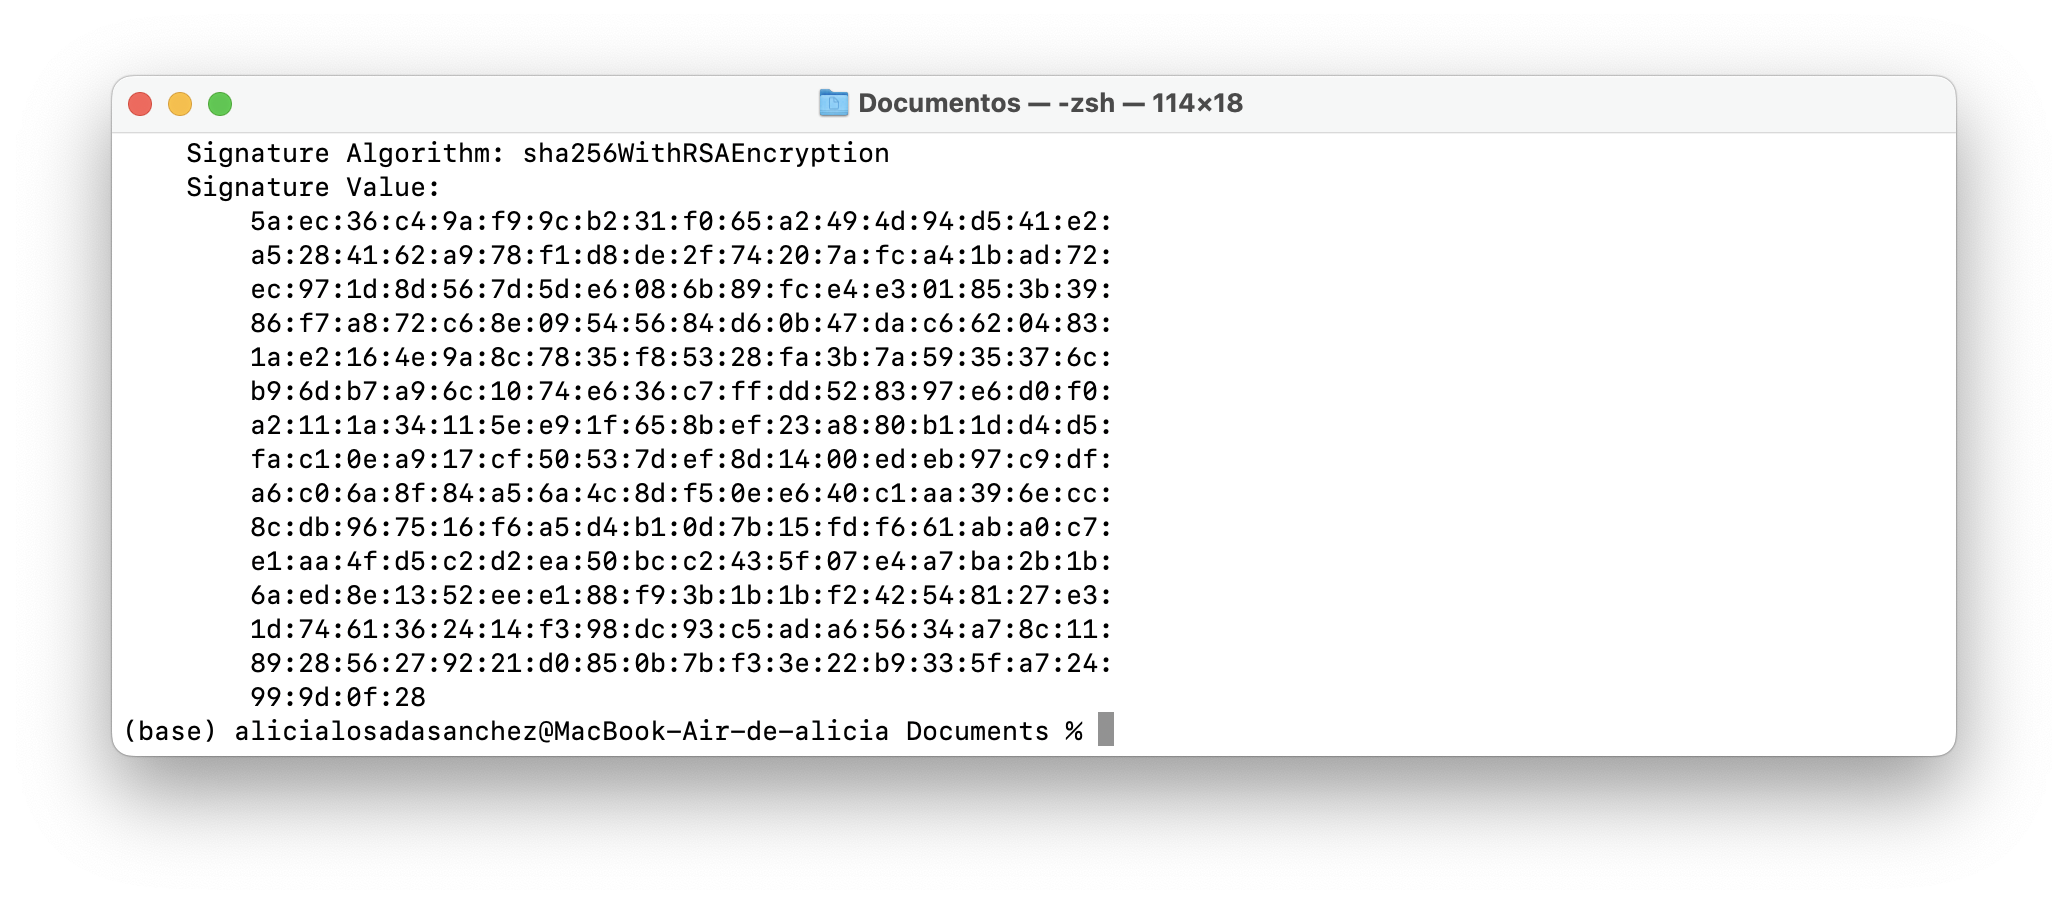
\includegraphics[width=0.8\textwidth]{apartadoc_3.png}
    \caption{Parte 3 campos clave pública}
    \label{fig:apartadoc_3}
\end{figure}

Una vez exportado el certificado digital en formato \texttt{.pem}, se ha utilizado la herramienta \texttt{OpenSSL} para examinar su contenido mediante el siguiente comando:


\begin{minted}[
    frame=single,
    framesep=8pt,
    breaklines,
    bgcolor=bgGray
]{bash}
    openssl x509 -in certificado_alicia.pem -noout -text
\end{minted}



En las Figuras \ref{fig:apartadoc_1}, \ref{fig:apartadoc_2} y \ref{fig:apartadoc_3} se pueden ver los distintos campos del certificado correspondiente.

A continuación, se detallan los campos más relevantes obtenidos del análisis:

\textbf{Versión y algoritmo de firma} \ Versión: 3 (X.509v3), lo que permite incluir extensiones adicionales. \ Algoritmo de firma: \texttt{sha256WithRSAEncryption}, que combina la función hash SHA-256 con el algoritmo RSA. Esta combinación garantiza la integridad y autenticidad del certificado.

\textbf{Número de serie} \ El número de serie del certificado es \texttt{11:22:51:08:ae:14:ec:78:67:ff:75:f1:ae:f3:ff:c2}. Este valor es único para cada certificado emitido por la autoridad certificadora y permite su identificación.

\textbf{Emisor (Issuer)} \ \texttt{C=ES, O=FNMT-RCM, OU=Ceres, CN=AC FNMT Usuarios} \ Este campo identifica a la Autoridad de Certificación (CA) que ha emitido el certificado: la Fábrica Nacional de Moneda y Timbre – Real Casa de la Moneda (FNMT-RCM), a través de la unidad AC FNMT Usuarios.

\textbf{Sujeto (Subject)} \ \texttt{C=ES, serialNumber=IDCES-49204290E, GN=ALICIA, SN=LOSADA SANCHEZ, CN=LOSADA SANCHEZ ALICIA} \ Indica la identidad del titular del certificado, incluyendo su NIF, nombre y apellidos.

\textbf{Periodo de validez} \ Not Before: 16 de abril de 2025 \ Not After: 16 de abril de 2029 \ El certificado tiene una vigencia de cuatro años. Durante ese tiempo se considera válido, salvo que sea revocado previamente.

\textbf{Clave pública} \ Algoritmo: RSA (2048 bits) \ Módulo: número entero de 2048 bits que constituye la base criptográfica de RSA. Es el producto de dos números primos grandes y debe mantenerse público. \ Exponente: 65537 (valor estándar ampliamente utilizado). \ El par \texttt{(módulo, exponente)} conforma la clave pública del titular. Esta clave se utiliza para verificar firmas digitales o cifrar datos dirigidos al propietario del certificado.

\textbf{Extensiones del certificado (X.509 v3)}

\begin{itemize}

    \item \textbf{Subject Alternative Name}: incluye información adicional sobre el titular, como su NIF, nombre y apellidos, codificados mediante OIDs específicos.

    \item \textbf{Basic Constraints (critical)}: \texttt{CA:FALSE}. Este certificado no puede actuar como autoridad certificadora.

    \item \textbf{Key Usage (critical)}: especifica los usos permitidos de la clave: firma digital, no repudio y cifrado de claves. Al estar marcado como \texttt{critical}, cualquier aplicación que no entienda este campo deberá rechazar el certificado.

    \item \textbf{Extended Key Usage}: indica que el certificado está destinado a la autenticación de cliente en servicios como páginas web seguras (TLS Web Client Authentication).

    \item \textbf{Subject Key Identifier} y \textbf{Authority Key Identifier}: permiten enlazar este certificado con el de su emisor dentro de una cadena de certificación.

    \item \textbf{Authority Information Access}: proporciona URLs para acceder a servicios de validación como OCSP (protocolo de comprobación del estado del certificado en tiempo real) y para descargar el certificado de la CA emisora.

    \item \textbf{Certificate Policies} y \textbf{CPS (Certification Practice Statement)}: contienen referencias a los documentos que regulan la emisión y el uso del certificado. Se especifica que se trata de un certificado cualificado de firma electrónica conforme a la legislación española.

    \item \textbf{CRL Distribution Points}: indica la ubicación de la lista de certificados revocados (CRL), que permite verificar si el certificado ha sido invalidado antes de su fecha de expiración.

\end{itemize}

\textbf{Fingerprint (huella digital)} \ El certificado incluye una huella digital generada mediante SHA-256. Esta huella permite identificar de manera única el certificado y detectar cualquier alteración de su contenido.

\textbf{Firma digital del certificado} \ El certificado está firmado por la FNMT utilizando el algoritmo \texttt{sha256WithRSAEncryption}. Esta firma permite a cualquier entidad comprobar que el certificado ha sido emitido por la FNMT y que no ha sido modificado.

\textbf{Cadena de certificación} \ Este certificado forma parte de una cadena de confianza que comienza en una Autoridad Certificadora raíz. Gracias a los campos \texttt{Authority Key Identifier} y \texttt{Authority Information Access}, es posible verificar su validez siguiendo la jerarquía de certificación.
